\documentclass[12pt , a4paper]{article}




\usepackage[a4paper, total={6in, 10in}]{geometry}


\usepackage{makecell}
\usepackage[utf8]{inputenc}
\usepackage{amsmath}
\usepackage{amsfonts}
\usepackage{amssymb}

\usepackage{graphicx}

\usepackage{fancyhdr}
\pagestyle{fancyplain}
\fancyhf{}
\renewcommand{\headrulewidth}{0pt} % remove lines as well

%font
\usepackage[T1]{fontenc}
\usepackage{uarial}
\renewcommand*{\familydefault}{\sfdefault}

%\setlength{\parskip}{10pt plus 1pt minus 1pt}

\usepackage{tabularx}

\author{Bardia Jedi}

\title{CV}


\begin{document}
	\begin{center}
	{\LARGE \textbf{CV}}
	\end{center}
	
	%contact info
	%contact info
	%img
	%\vspace{-12pt}
	\makebox[0pt][l]{%
 	\raisebox{-\totalheight}[-1pt][-1pt]{%
    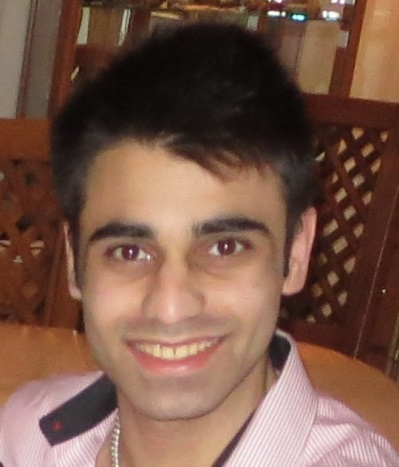
\includegraphics[width=30mm]{pimg01.jpg}}}%
	
	\begin{tabularx}{\textwidth}{ l X r  }				
  		 			&& 
  			\begin{tabular}{ r  l }
					&	\textbf{Bardia Jedi}\\
							%&\\				
					&	Kakelösagatan 3\\
					&	43144 MÖLNDAL\\  
							%&\\				
  					& 0768-957983\\
  					& bardiajedi@gmail.com \\
 
			\end{tabular}\\
	\end{tabularx}

	\begin{flushleft}
	
		%profile
		\vspace{24pt}
		\vspace{24pt}
		{\large \textbf{Personlig Profil}}
		\hrule		
		
		\vspace{12pt}
		\textbf{Ansvarsfull} – Att ta ansvar på största allvar på arbetsplatsen är givet och jag gör alltid mitt bästa för att få resultat.

			\vspace{3 pt}
	    	\textbf{Entusiastisk} - Jag har alltid varit postiv med det jag har jobbat med.
	    	På detta sätt försöker jag att sprida glädje i omgivningen.
	    	
	    	
			\vspace{3 pt}
 		    \textbf{Social} - Jag har alltid lätt att få kontakt med människor.	
			
			
			\vspace{3 pt}
 		    \textbf{Problemlösare} - Lösa problem är min hobby (problem = pussel, matematik, social, etc.),det glädjer mig när jag löser ett problem. Jag är öppen till sinnet när det gäller problem, alltid redo för nya idéer och inspiration. 
		
		\vspace{12pt}		
		{\large \textbf{Arbetslivserfarenhet}}
		\hrule
		\vspace{6pt}
				
		\textbf{Lärarvikarie: } 2011 - 2012	
		
		%\vspace{3pt}
		Under denna period har jag varit med ÅK 1-9 och undervisat för Mölndals kommun.
		Mitt uppdrag var bland annat at vara hjälplärare, idrottslärare och fritidsledare.
		
		\vspace{6pt}
		\textbf{Köksbiträde: } 2009
		
		%\vspace{3pt}
		%Där bodde jag och jobbad som köks betred i en restrung
		Bodde i London under sommaren och arbetade på en restaurang. 
		
		%edu
		\vspace{12pt}
		{\large \textbf{Utbildningar}}
		\hrule
		
		
		% sptare the eduction
		\vspace{6pt}
		
		 \textbf{Blekinge Tekniska Högskola: } 2012 - 2013. 
		
		\vspace{3pt}
				
		Under denna period studerade jag software engineering på BTH,
		vilket innehöll behärskning av programmeringsspråk , databashantering, OS, etc. 
		
		
		För tillfälle har jag tagit studieuppehåll.
		
		\vspace{6pt}
		
		\textbf{Fässbergsgymnasiet: }Teknik, 2008 - 2011


	
		
		%Språk
		\vspace{12pt}
		{\large \textbf{Språk}}
		\hrule
		\vspace{12pt}

		\textbf{Engelska}, Flytande tal och skrift
		
		\textbf{Persiska} (Farsi), Flytande 

		\textbf{Svenska}, Flytande
		
		%computer konwlege LoL
		\vspace{12pt}
		{\large \textbf{Datorkunskaper}}
		\hrule
		\vspace{12pt}
		Jag har mycket goda kunskaper i MS Office, LiberOffice, Adobe Photoshop, GIMIP och LaTeX(PDF).
		\vspace{6pt}		
		\hrule
		\vspace{6pt}		
		
		Referenser lämnas på begäran

	\end{flushleft}		
	
	

\end{document}

